\documentclass[letterpaper,12pt,listof=totoc]{scrartcl}
%------------------------------------------------
%   PACKAGES FOR LAYOUT AND FONTS
%------------------------------------------------
%------------------------------------------------
% % PAGE LAYOUT & ENCODING
%------------------------------------------------
% This uses the simpler 'margin=1in' from your second example.
% Your first example had: [tmargin=2cm,rmargin=1in,lmargin=1in,margin=0.85in,bmargin=2cm,footskip=.2in]
\usepackage[margin=1in]{geometry} 
\usepackage[utf8]{inputenc}
\usepackage[T1]{fontenc}
\usepackage{lmodern} % Better font than default
\usepackage[english]{babel}
\usepackage{microtype} % Improves text spacing

%------------------------------------------------
% % MATH & SYMBOLS PACKAGES
%------------------------------------------------
\usepackage{amsmath,amsfonts,amsthm,amssymb} % Core math
\usepackage{mathtools} % Extensions for amsmath
\usepackage{xfrac} % Slanted fractions (sfrac)
\usepackage[makeroom]{cancel} % Cancel terms in equations
\usepackage{bm} % Bold math symbols
\usepackage{bbm} % Blackboard bold (e.g. \mathbbm{1})
\usepackage{stmaryrd} % More symbols
\usepackage{physics} % Common physics/math commands
\usepackage{siunitx} % Units and scientific notation
\usepackage{mhchem} % Chemistry formulas

%------------------------------------------------
% % GRAPHICS, COLOR & BOXES
%------------------------------------------------
\usepackage{xcolor}
  \newcommand\cave[1]{\textcolor{red}{#1}}
\usepackage{graphicx}
\usepackage[export]{adjustbox}
\usepackage{subcaption} % For subfigures
\usepackage{tikz}
\usepackage{tikz-cd} % Commutative diagrams
\usepackage{tikzsymbols}
\usetikzlibrary{patterns,arrows.meta,calc,decorations.pathreplacing}
\usepackage[most,many,breakable]{tcolorbox}
\usepackage{float}

%------------------------------------------------
% % LISTS, TABLES & ALGORITHMS
%------------------------------------------------
\usepackage{enumitem} % Advanced list customization
\usepackage{multicol,array}
\usepackage[ruled,vlined,linesnumbered]{algorithm2e}

%------------------------------------------------
% % FILE & DOCUMENT UTILITIES
%------------------------------------------------
\usepackage{subfiles} % For multi-file projects
\usepackage{import}
\usepackage{pdfpages} % Include PDF pages
\usepackage{comment} % Multi-line comments
\usepackage{etoolbox} % Programming tools
\usepackage{xifthen} % Conditional commands
\usepackage{varwidth} % Box with variable width
\usepackage{transparent}
%\usepackage{authblk} % Commented out as in your original

%------------------------------------------------
% % HEADER, FOOTER & PAGE STYLE
%------------------------------------------------
\usepackage{fancyhdr}
\pagestyle{fancyplain}
\fancyhead{}
\fancyfoot[L]{}
\fancyfoot[C]{}
\fancyfoot[R]{\thepage}
\renewcommand{\headrulewidth}{0pt}
\renewcommand{\footrulewidth}{00pt}
\setlength{\headheight}{13.6pt}

%------------------------------------------------
% % THEOREM ENVIRONMENTS
%------------------------------------------------
\newtheorem{theorem}{Theorem}[section]
\newtheorem{lemma}[theorem]{Lemma}
\newtheorem{proposition}[theorem]{Proposition}
\newtheorem{corollary}[theorem]{Corollary}
\theoremstyle{definition}
\newtheorem{definition}[theorem]{Definition}
\newtheorem{example}[theorem]{Example}
\theoremstyle{remark}
\newtheorem{remark}[theorem]{Remark}

%------------------------------------------------
% % NUMBERING
%------------------------------------------------
\numberwithin{equation}{section}
\numberwithin{figure}{section}
\numberwithin{table}{section}

%------------------------------------------------
% % CUSTOM COMMANDS
%------------------------------------------------

%------------------------------------------------
% % HYPERLINKS & REFERENCES (Load Near End)
%------------------------------------------------
\usepackage{hyperref}
\usepackage{theoremref} % Must load after amsthm and hyperref
\usepackage{bookmark} % Better PDF bookmarks
\usepackage{nameref} % Reference sections by name
\definecolor{darkblue}{rgb}{0,0,0.5}
\definecolor{darkred}{rgb}{0.5,0,0}

\hypersetup{
    pdftitle={Assignment},
    colorlinks=true,
    linkcolor=darkred,    % Internal (Goes to section/eq)
    citecolor=darkred,    % Citations (Goes to bibliography)
    urlcolor=darkblue,    % External (Goes to web)
    bookmarksnumbered=true,
    bookmarksopen=true
}

\usepackage{varioref}

\usepackage{listings}

\lstdefinelanguage{Julia}{
  keywords={function, end, return, for, while, if, else, elseif, mutable, struct},
  keywordstyle=\color{blue}\bfseries,
  comment=[l]\#,
  commentstyle=\color{gray},
  stringstyle=\color{red},
}

\lstset{
  language=Julia,
  basicstyle=\ttfamily\small,
  numbers=left,             % ← line numbers
  numberstyle=\tiny\color{gray},
  stepnumber=1,
  numbersep=8pt,            
  breaklines=true,          % ← wrap long lines
  breakatwhitespace=false,
  columns=fullflexible,     % better wrapping
  showstringspaces=false,
  mathescape=true,
  escapeinside={(*@}{@*)},
  literate=
    {θ}{{$\theta$}}1
    {Θ}{{$\Theta$}}1
    {Δ}{{$\Delta$}}1
    {ω}{{$\omega$}}1
    {Ω}{{$\Omega$}}1
}

\input{letterfonts.tex}
\input{macros.tex}
\usepackage{setspace}
\usepackage[nottoc]{tocbibind} % Automatically adds bib to TOC
\rhead{Double Pendulum}
\renewcommand{\sectionmark}[1]{\markright{\thesection\ #1}} %%Left header command
\lhead{\nouppercase{$\S$\rightmark}} %%Left header
\renewcommand{\headrulewidth}{0.4pt}


%------------------------------------------------
%   DOCUMENT BODY
%------------------------------------------------
\begin{document}

\begin{titlepage}
	
	\centering
	
	{\large\textsc{University of Utah, Mathematics Department}} % Publisher
	\rule{\textwidth}{1pt} % Thick horizontal rule
	
	\vspace{2pt}\vspace{-\baselineskip} % Whitespace between rules
	
	\rule{\textwidth}{0.4pt} % Thin horizontal rule
	
	\vspace{0.05\textheight} % Whitespace between the top rules and title
	
	%------------------------------------------------
	%	Title
	%------------------------------------------------
	
		{\Huge CHAOTIC MOTION}\\[0.5\baselineskip]
		{\Large IN}\\[0.5\baselineskip] % Title line 2
    {\Huge DOUBLE PENDULUM SYSTEMS}\\[1.0\baselineskip]
	{\Large A Final Computing Project}
	\vspace{0.025\textheight} % Whitespace between the title and short horizontal rule
	
	\rule{0.75\textwidth}{0.4pt} % Short horizontal rule under the title
	
	\vspace{0.05\textheight} % Whitespace between the thin horizontal rule and the author name
	
	%------------------------------------------------
	%	Author
	%------------------------------------------------
	
{\Large Charles Godfrey \qquad Tannon Warnick \qquad Henry Whiting}\\[1.5\baselineskip]
\begin{abstract}
\begin{center}
  \textbf{Abstract} 
\end{center}
  This abstract was generated by Gemini  based on this papers content \cite{gemini}.
This project investigates the nonlinear and chaotic dynamics of a double pendulum system. Starting from the Lagrangian formulation, we derive the coupled second-order differential equations governing the system’s motion. These equations are then transformed into a first-order state-space representation suitable for numerical integration. Using a fourth-order Runge–Kutta (RK4) method implemented in Julia, we simulate the motion and analyze the system’s sensitivity to initial conditions. Numerical experiments demonstrate infinitesimal perturbations in the initial angles lead to exponentially divergent trajectories. The results illustrate how a physically simple, deterministic system can exhibit rich, unpredictable behavior.\end{abstract}
	\vfill % Whitespace between the author name and publisher
	
	%------------------------------------------------
	%	Publisher
	%------------------------------------------------
	\includegraphics[width=0.2\textwidth]{U_medallion_BLACK.png}
	\vspace{0.1\textheight} % Whitespace under the publisher text
	
	%------------------------------------------------
	%	Bottom rules
	%------------------------------------------------
	{\Large \today}
	\rule{\textwidth}{0.4pt} % Thin horizontal rule
	
	\vspace{2pt}\vspace{-\baselineskip} % Whitespace between rules
	
	\rule{\textwidth}{1pt} % Thick horizontal rule
\end{titlepage}
\pagenumbering{roman}
\thispagestyle{empty}
\tableofcontents
\listoffigures
\clearpage
\pagenumbering{arabic}
\newpage
\setcounter{page}{1}
\section{Introduction}
A single pendulum is a classical example of simple harmonic motion. When constrained to small angles the pendulum will swing periodically and consistently. They are so predictable that some have been used to keep time. By simply adding a second pendulum at the end of the first, the system transforms into a classical example of chaotic motion. Even though these two systems are governed by the same physical laws of motion and only being acted upon by one force (gravity), a double pendulum is \emph{heavily} dependent on initial conditions. We will use an approximation to solve this equation to view the behavior; the approximation we will use is the fourth order Runge-Kutta method.

\section{Mathematical Model}

We must first derive the equations of motion. Because the system involves multiple degrees of freedom, the Lagrangian formulation of mechanics is significantly more efficient than the Newtonian approach \cite{taylor}.

\subsection{System Setup and Geometry}

We consider a system of two point masses, $m_1$ and $m_2$, connected by massless rigid rods of length $l_1$ and $l_2$. The system is confined to a 2D plane and acted upon by a uniform gravitational field $g$ pointing downwards. The system can be visualized in \figref{system}. Note: unlike in \shortfigref{system}, the mathematical (and numerical) system will not intersect with itself or other objects.

\begin{figure}[h]
\begin{center}
  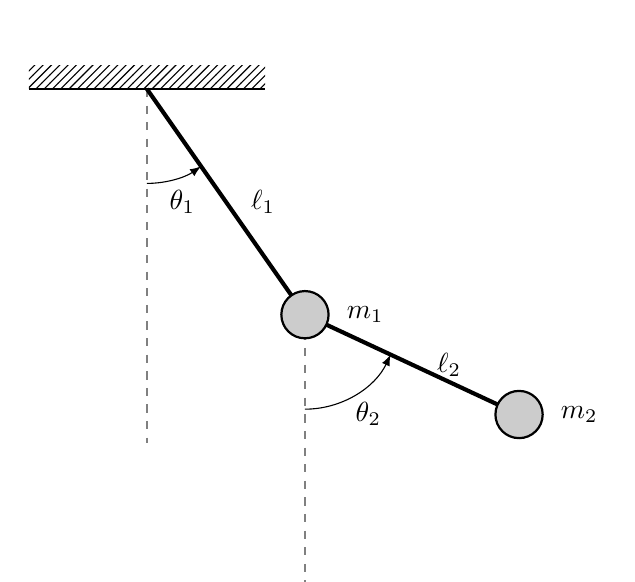
\begin{tikzpicture}[>=latex, thick]
    % --- Definitions ---
    \def\Lone{3.5}
    \def\Ltwo{3}
    \def\angOne{35}  % Theta 1
    \def\angTwo{65}  % Theta 2
    \def\massR{0.3}
    \def\arcR{1.2}   % Radius of the angle arcs

    % --- Coordinates ---
    \coordinate (O) at (0,0);
    \coordinate (M1) at ({\angOne-90}:\Lone);
    \coordinate (M2) at ($(M1) + ({\angTwo-90}:\Ltwo)$);

    % --- Ceiling ---
    \draw[thick] (-1.5,0) -- (1.5,0);
    \fill[pattern=north east lines] (-1.5,0) rectangle (1.5,0.3);

    % --- Vertical Reference Lines ---
    \draw[dashed, gray] (O) -- (0,-4.5);
    \draw[dashed, gray] (M1) -- ++(0,-3.5);

    % --- Rods ---
    \draw[line width=1.5pt] (O) -- (M1) node[midway, right=5pt] {$\ell_1$};
    \draw[line width=1.5pt] (M1) -- (M2) node[midway, right=5pt] {$\ell_2$};

    % --- Masses ---
    \filldraw[fill=gray!40] (M1) circle (\massR) node[right=0.4cm] {$m_1$};
    \filldraw[fill=gray!40] (M2) circle (\massR) node[right=0.4cm] {$m_2$};

    % --- FIXED ANGLES ---
    % Using '++' ensures the arc is anchored exactly to the pivot point
    
    % Theta 1
    % Move to O, shift down by arcR, then draw arc
    \draw[->, thin] (O) ++(-90:\arcR) arc (-90:{\angOne-90}:\arcR);
    \node at ({\angOne/2 - 90}:\arcR+0.3) {$\theta_1$};

    % Theta 2
    % Move to M1, shift down by arcR, then draw arc
    \draw[->, thin] (M1) ++(-90:\arcR) arc (-90:{\angTwo-90}:\arcR);
    % Label calculation is relative to M1
    \path (M1) ++({\angTwo/2 - 90}:\arcR+0.3) node {$\theta_2$};

\end{tikzpicture}
\end{center}
\caption{Double pendulum system}
\figlabel{system}
\end{figure}

The system we will construct mathematically, and which is depicted in \shortfigref{system}, is a simple pendulum. A compound pendulum can be similarly derived by just substituting the positions of the point masses with the positions of the centers of mass \cite{wikidp}.

We define the generalized coordinates as the angles $\theta_1$ and $\theta_2$, measured from the vertical axis. The origin is the pivot point of the first pendulum. This will be easier to compute mathematically, and therefore numerically than the Cartesian system, although it is easier to visualize as such.
\begin{align}
  x_1 &= \ell_1 \sin \theta_1 \\
    y_1 &= -\ell_1 \cos \theta_1 \\
    x_2 &=\ell_1\sin\theta_1+\ell_2\sin\theta_2\\
    y_2 &= - \ell_1\cos \theta_1+\ell_2\cos\theta_2
\end{align}

\subsection{The Lagrangian Formulation}

The Lagrangian $\mathcal{L}$ is defined as the difference between the kinetic energy ($T$) and the potential energy ($V$) of the system:
\[ \mathcal{L} = T - V \]

\subsubsection{Kinetic Energy ($T$)}
The kinetic energy of the system is the sum of the kinetic energies of the masses:
\[ T = \frac{1}{2}m_1 v_1^2 + \frac{1}{2}m_2 v_2^2 \]
Calculating the velocities squared ($v^2 = \dot{x}^2 + \dot{y}^2$):
\begin{align*}
    v_1^2 &= (l_1 \dot{\theta}_1)^2 \\
    v_2^2 &= \dot{x}_2^2 + \dot{y}_2^2 \\
          &= l_1^2 \dot{\theta}_1^2 + l_2^2 \dot{\theta}_2^2 + 2 l_1 l_2 \dot{\theta}_1 \dot{\theta}_2 (\sin \theta_1 \sin \theta_2 + \cos \theta_1 \cos \theta_2) \\
          &= l_1^2 \dot{\theta}_1^2 + l_2^2 \dot{\theta}_2^2 + 2 l_1 l_2 \dot{\theta}_1 \dot{\theta}_2 \cos(\theta_1 - \theta_2)
\end{align*}
Thus, the total kinetic energy is:
\begin{equation}
    T = \frac{1}{2}(m_1 + m_2) l_1^2 \dot{\theta}_1^2 + \frac{1}{2}m_2 l_2^2 \dot{\theta}_2^2 + m_2 l_1 l_2 \dot{\theta}_1 \dot{\theta}_2 \cos(\theta_1 - \theta_2)
\end{equation}

\subsubsection{Potential Energy ($V$)}
Assuming potential energy is zero at $y=0$, we have:
\begin{align}
    V &= m_1 g y_1 + m_2 g y_2 \nonumber \\
      &= -(m_1 + m_2) g l_1 \cos \theta_1 - m_2 g l_2 \cos \theta_2
\end{align}

\subsection{Equations of Motion}
Applying the Euler-Lagrange equation for each coordinate $\theta_i$:
\[ \frac{d}{dt}\left(\frac{\partial \mathcal{L}}{\partial \dot{\theta}_i}\right) - \frac{\partial \mathcal{L}}{\partial \theta_i} = 0 \]

Solving these derivatives yields a system of two, non-linear second-order differential equations.

For $\theta_1$:
\begin{equation}\label{theta1}
    (m_1 + m_2) l_1 \ddot{\theta}_1 + m_2 l_2 \ddot{\theta}_2 \cos(\theta_1 - \theta_2) + m_2 l_2 \dot{\theta}_2^2 \sin(\theta_1 - \theta_2) + (m_1 + m_2) g \sin \theta_1 = 0
\end{equation}

For $\theta_2$:
\begin{equation}\label{theta2}
    m_2 l_2 \ddot{\theta}_2 + m_2 l_1 \ddot{\theta}_1 \cos(\theta_1 - \theta_2) - m_2 l_1 \dot{\theta}_1^2 \sin(\theta_1 - \theta_2) + m_2 g \sin \theta_2 = 0
\end{equation}

These two equations completely describe the motion of the double pendulum. In Section 3, we will rearrange these terms to solve for $\ddot{\theta}_1$ and $\ddot{\theta}_2$ explicitly to implement the RK4 algorithm.

\section{Numerical Model}
The full Julia code used to execute this method used in this derivation can be found in \appref{A}.

\section{Results and Discussion}

Using what we have established in previous sections provides the necessary tools to simulate the double pendulum's complex dynamics. With the equations of motion derived via the Lagrangian and the Runge-Kutta solver implemented in Julia, we now turn to the simulation results.

\subsection{Numerical Results}
To verify the chaotic nature of the double pendulum, we simulated the system's time evolution using the RK4 integrator derived in Section 3. We specifically investigated the system's sensitivity to initial conditions.

We initialized two \textit{almost} identical double pendulum systems (sharing identical lengths $l_1,l_2$ and masses $m_1,m_2$) with initial angles differing by a microscopic perturbation, $\epsilon$:
\[\Theta_A=(\theta_1,\theta_2)\quad\text{and}\quad \Theta_B=(\theta_1+\epsilon,\theta_2)\]
where $\epsilon = 10^{-5}$ degrees.

\figref{10-5} illustrates the trajectories of these two systems over time. During the initial phase of the simulation, the deviation caused by the perturbation appears negligible, and the systems move in unison. However, as the system evolves, the non-linear coupling terms in the equations of motion, specifically those derived in \eqref{eq:rearr1}, cause this infinitesimal difference $\epsilon$ to propagate and grow exponentially for some time.

\begin{figure}[h]
  \centering
    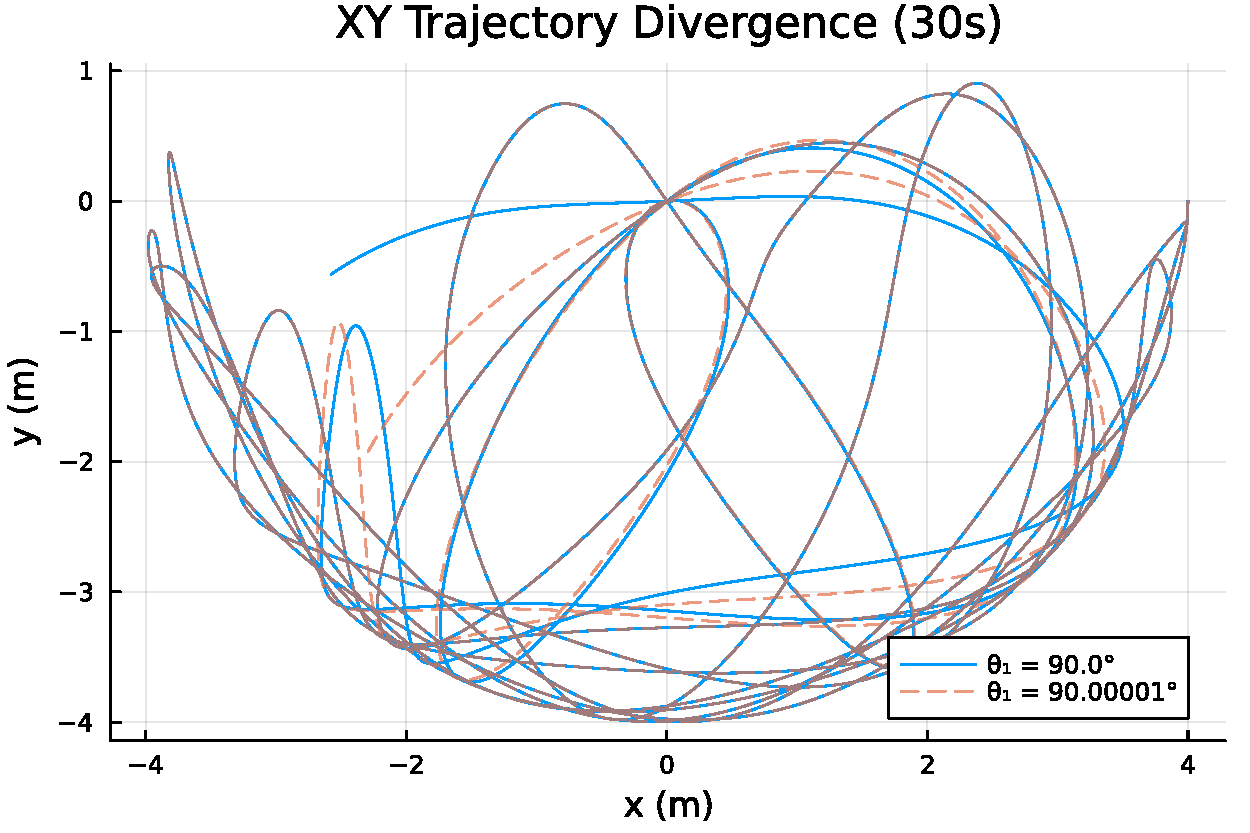
\includegraphics[width=0.8\textwidth]{Figures/xy_divergence.pdf}
    \caption{Divergence of trajectories with initial conditions differing by $10^{-5}$ degrees.}
    \figlabel{10-5}
\end{figure}

By the end of the simulation, the two pendulums exhibit completely uncorrelated states, occupying different regions of the configuration space despite being governed by the same deterministic laws. This confirms that while the double pendulum is deterministic (fully described by Equations \ref{ddtheta1} and \ref{ddtheta2}), it is practically unpredictable over long time horizons due to this extreme sensitivity.

Plotting the angular difference $\Delta\theta$ between the two systems further illustrates this chaotic dissociation. As shown in \figref{dt}, the error does not grow linearly but exhibits rapid, unpredictable fluctuations, the peaks of which grow exponentially, characteristic of the butterfly effect.

\begin{figure}[h]
  \centering
    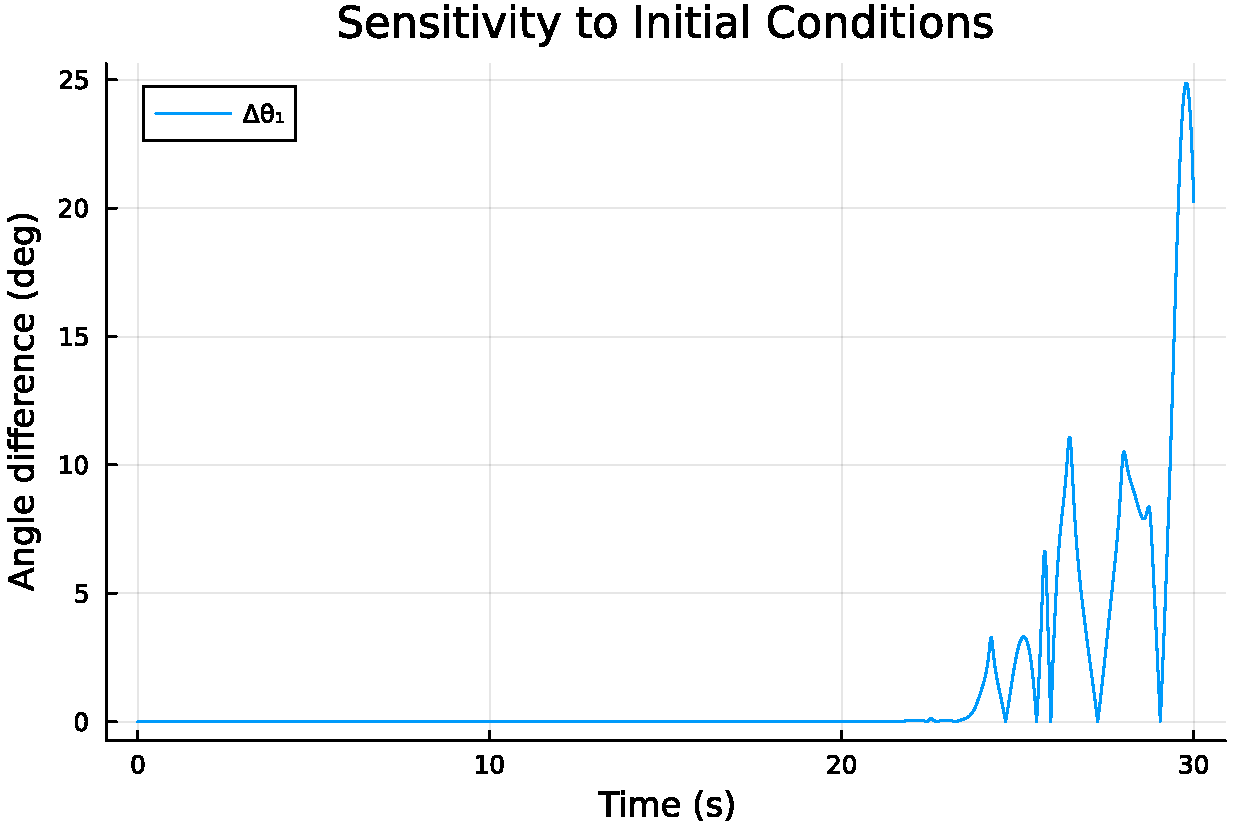
\includegraphics[width=0.8\textwidth]{Figures/dt.pdf} 
    \caption{Evolution of the angular difference $\Delta\theta$ between the two systems over time.}
    \figlabel{dt}
\end{figure}

\subsection{Conclusion}
In this project, we modeled the dynamics of a double pendulum, moving from the theoretical physical setup to a full numerical simulation. By utilizing the Lagrangian formulation, we avoided the vector complexity of Newtonian mechanics and directly derived the coupled non-linear equations of motion.

We transformed these second-order differential equations into a state-space representation suitable for computational solving. The implementation of the fourth-order Runge-Kutta (RK4) method allowed us to accurately approximate the solution, maintaining numerical stability even as the system entered chaotic regimes.

The results validate that simple physical systems can exhibit complex, non-linear behavior. The visualization of the trajectory divergence serves as a concrete demonstration of deterministic chaos, satisfying the primary objective of this study. Future work could involve solving triple or \(n\)-pivot pendulums. This would require much higher dimension vector fields to incorporate into the Runge-Kutta methods. 


\appendix\section{Julia Code}
\applabel{A}

Here is the compilation of all Julia code needed to solve the system in this paper.
\begin{lstlisting}
using Plots
gr()  # Set plotting backend

# parameters
G = 9.8
lengths = [2.0, 2.0]
masses = [2.0, 2.0]
time_span = (0.0, 30.0)  # 30 seconds
n_steps = 15000           # RK4 steps

# =================== RK4 Solver =================== #
function rk4(IVP, n)
    a, b = IVP.tspan
    h = (b - a)/n
    t = [a + i*h for i in 0:n]

    u0 = IVP.u0
    m = length(u0)
    u = zeros(m, n+1)
    u[:,1] .= u0

    for i in 1:n
        k1 = h * IVP.f(u[:,i], IVP.p, t[i])
        k2 = h * IVP.f(u[:,i] + k1/2, IVP.p, t[i] + h/2)
        k3 = h * IVP.f(u[:,i] + k2/2, IVP.p, t[i] + h/2)
        k4 = h * IVP.f(u[:,i] + k3, IVP.p, t[i] + h)
        u[:,i+1] = u[:,i] + (k1 + 2*k2 + 2*k3 + k4)/6
    end

    return t, u
end

# Double Pendulum ODE (returns vector)
function double_pendulum(u, p, t)
    m1, m2, l1, l2, g = p
    theta1, omega1, theta2, omega2 = u

    Delta = theta2 - theta1
    denom1 = (m1 + m2)*l1 - m2*l1*cos(Delta)^2
    denom2 = (l2/l1)*denom1

    du = zeros(4)
    du[1] = omega1
    du[2] = ( m2*l1*omega1^2*sin(Delta)*cos(Delta) +
              m2*g*sin(theta2)*cos(Delta) +
              m2*l2*omega2^2*sin(Delta) -
              (m1+m2)*g*sin(theta1) ) / denom1

    du[3] = omega2
    du[4] = ( -m2*l2*omega2^2*sin(Delta)*cos(Delta) +
              (m1+m2)*g*sin(theta1)*cos(Delta) -
              (m1+m2)*l1*omega1^2*sin(Delta) -
              (m1+m2)*g*sin(theta2) ) / denom2

    return du
end

# IVP Struct 
struct ODEProblem
    f::Function
    u0::Vector{Float64}
    tspan::Tuple{Float64, Float64}
    p::Tuple
end

# Simulation Function
function simulate_pendulum(theta1_deg, theta2_deg; omega1=0.0, omega2=0.0)
    u0 = deg2rad.([theta1_deg, omega1, theta2_deg, omega2])
    p = (masses[1], masses[2], lengths[1], lengths[2], G)
    IVP = ODEProblem(double_pendulum, u0, time_span, p)
    t, u = rk4(IVP, n_steps)
    return t, u
end

# Plotting Multiple Initial Conditions
initial_conditions = [
    (90.0, 90.0),
    (91.0, 90.0),
    (90.0, 91.0)
]

plot(title="Double Pendulum Theta vs Time", xlabel="Time (s)", ylabel="Angle (deg)")

for (theta1, theta2) in initial_conditions
    t, u = simulate_pendulum(theta1, theta2)
    plot!(t, rad2deg.(u[1,:]), label="theta1 start=($theta1,$theta2)")
    plot!(t, rad2deg.(u[3,:]), label="theta2 start=($theta1,$theta2)")
end

t, u1 = simulate_pendulum(90.0, 90.0)
t, u2 = simulate_pendulum(90.00001, 90.0)
x_vals = @. lengths[1] * sin(u[1,:]) + lengths[2] * sin(u[3,:])
y_vals = @. -lengths[1] * cos(u[1,:]) - lengths[2] * cos(u[3,:])

# Plotting Delta Theta graph
plot(t, rad2deg.(abs.(u1[1,:] .- u2[1,:])), label="Delta theta1", xlabel="Time (s)", ylabel="Angle difference (deg)", title="Sensitivity to Initial Conditions")

# Plotting (x,y) graph
plot(x_vals, y_vals, xlabel="x (m)", ylabel="y (m)", title="Pendulum Trajectory", aspect_ratio=:equal, label="")
\end{lstlisting}



% For References
\newpage
\begin{thebibliography}{9}

\bibitem{wikidp}
  Double pendulum
  \newblock \textit{Wikipedia}. 
\newblock \url{https://en.wikipedia.org/wiki/Double_pendulum}. 
\newblock Accessed: 2025-12-11.
\bibitem{taylor}
John R. Taylor.
\newblock \textit{Classical Mechanics}.
\newblock University Science Books, 2005.

  \bibitem{gemini}
Google.
\newblock \textit{Gemini} [Large Language Model].
\newblock \url{https://gemini.google.com}.
\newblock Accessed: 2025-12-11.
\end{thebibliography}\thispagestyle{empty}
\end{document}

